% sections/student_resumption.tex: the October 2023 student-loan payment resumption as a cross-loan timing experiment (E13, I11). Numbers filled from results/student_*.csv.
\subsection{Student Loans: The Statutory Payment Resumption}\label{sec:studentloan}

\paragraph{The design in summary.} The Fiscal Responsibility Act of 3 June 2023 fixed the date on which federal student-loan payments resumed, October 2023, and the size of each bill was fixed by the student loan; for the 324,586 holders in the panel who also hold an auto loan it is a payment increase on another account at a date fixed by statute four months in advance, at an auto balance that does not change. Auto default did not respond to it at any horizon. On 743,487 auto loans with 17,711 first 90-day delinquencies, the coefficient of delinquency on the resumed bill per hundred dollars, in units of $10^{-5}$ per month with loan and calendar-month fixed effects, is $-3.1$ before the statute, $-4.1$ in the four months between the statute and the first bill and $-5.9$ from October 2023, with standard errors between $0.5$ and $1.0$; the change at the bill is $-2.8$ ($0.6$), against the $+5.9$ that an enforced payment of that size would produce at the panel's payment elasticity, and no score tercile or income quartile has a positive coefficient before the bill, at it or after it (Table \ref{tab:student_groups}). The reason is that the bill was not a payment. By January 2024, 41 percent of the holders billed up to \$100 and 61 percent of those billed more than \$500 show a positive payment, the shares do not rise afterward, and under the twelve-month on-ramp a missed payment was not reported as delinquent until October 2024, so half of the resumed bills were unpaid and had no consequence within the window (Table \ref{tab:student_takeup}). Proposition \ref{prop:sensT} weights a payment by the probability that it is due, and a bill that half of its recipients set aside is not the known and binding payment of Remark \ref{rem:experimentsT}; the measured zero, within $\pm 1.4 \times 10^{-5}$ per month, two percent of the base hazard, is the model's response to an obligation that is not enforced. Appendix \ref{appendix:timing} reports the take-up, the monthly profile and the responses by group.

Federal student-loan payments were suspended in March 2020. The Fiscal Responsibility Act of 3 June 2023 fixed the end of the suspension: interest from 1 September and the first payment due in October 2023. For a borrower who also holds an auto loan, the resumption is a payment increase on another account at a date fixed by statute four months in advance, of a size fixed by the student loan's balance and plan, at an auto balance that does not change. It is the design of Remark \ref{rem:experimentsT} at scale: the one-percent panel holds 438,311 consumers with a student-loan balance in September 2023, of whom 324,586 hold an auto loan open in January 2023, and their auto loans record 17,711 first 90-day delinquencies over 2022 to mid-2025. The response of auto delinquency to the size of the resumed payment in June to September 2023, the four months between the statute and the first bill, relative to the response from October 2023, is the anticipation profile of Proposition \ref{prop:sensT} at horizons of four to one months, $D(\tau)Q_\tau\lambda$, and the borrowers whose resumed payment is zero on a positive balance, the income-driven plans, receive the same information and no payment.

\paragraph{The exposure and its take-up.} The median of the 438,311 holders (the bins of Table \ref{tab:student_takeup} cover the 429,918 with a bill observed) owed \$20,408 in September 2023 and was billed \$80 a month from November, with an interquartile range from zero to \$244; 34 percent of holders with a positive balance were billed nothing, the income-driven plans. The bill was not a payment. Table \ref{tab:student_takeup} follows the student trades' actual-payment field: by January 2024, 41 percent of the holders billed up to \$100 and 61 percent of those billed more than \$500 show a positive payment, the median payment among those billed \$100 to \$500 equals the bill, and the shares do not rise afterward. Under the Department of Education's twelve-month on-ramp, missed payments were not reported as delinquent until October 2024, and the share of holders with a past-due student balance stays between two and four percent through January 2025. Half of the resumed bills were paid and the other half had no consequence within the window.

\paragraph{The response.} Figure \ref{fig:student_profile} reports, for each month from March 2023 to December 2025, the coefficient of first 90-day (and 60-day) auto delinquency on the resumed monthly bill in hundreds of dollars, with loan and calendar-month fixed effects and January 2022 to February 2023 as the reference, on 743,487 auto loans open in January 2023 and 17,711 first 90-day events. The coefficients, times $10^{5}$, are $-3.1$ in March to May 2023, before the statute, $-4.1$ in the four months between the statute and the first bill, $-5.9$ in October to December 2023, near $-6$ through 2024, and $-5.7$ from May 2025, when collection resumed, with standard errors between $0.5$ and $1.0$. The base hazard is $0.066$ percent per month. The response an enforced payment of the same size would produce is the panel's elasticity applied to the auto payment: a \$100 bill against a median auto payment near \$500 is a fifth of the obligation, and at the elasticity of $0.45$ the coefficient would be $+5.9$. The measured coefficient is negative at every month, is negative before the statute, and changes between the pre-statute months and the bill months by $-2.8$ ($0.6$). The sign is the composition of the exposure, not a response: a larger bill is a larger balance, which is more education and a lower and falling auto-delinquency hazard over 2023 to 2025, and the fixed effects remove the level but not the drift. Table \ref{tab:student_groups} reports the same three windows by score tercile and income quartile: no group has a positive coefficient before the bill, at it, or after it, and the bottom score tercile, with 13,837 events, has $-3$ ($1$) before and $-6$ ($2$) at the bill.

\paragraph{What the resumption establishes.} Proposition \ref{prop:sensT} weights a future payment by the probability that it is due, and a bill that half of its recipients do not pay and that has no consequence for a year is due with a probability that the design does not fix. The resumption therefore does not meet the premise of Remark \ref{rem:experimentsT}, a known and binding payment, at the enforcement margin, and its zero is the model's zero for an obligation the borrower can set aside: the response of auto default to \$100 of unenforced bill on another account is measured to within $\pm 1.4\times 10^{-5}$ per month, two percent of the base hazard, and is not positive at any horizon in any group. What remains open is the response to the enforced payments after mid-2025, which the coefficients from May to December 2025 do not distinguish from the preceding drift, and which a longer panel will measure. The two timing designs the bureau offers in this period, the resets and the resumption, are both found and both measured, and neither delivers the discount function: the resets for want of exogenous variation in size and of events, the resumption for want of an enforced payment. Appendix \ref{appendix:strategies} records both, and the discount rate the paper reports comes from the experiments of Section \ref{sec:quasi}, whose payment changes were enforced and whose sizes were assigned.

\begin{figure}[H]
\centering
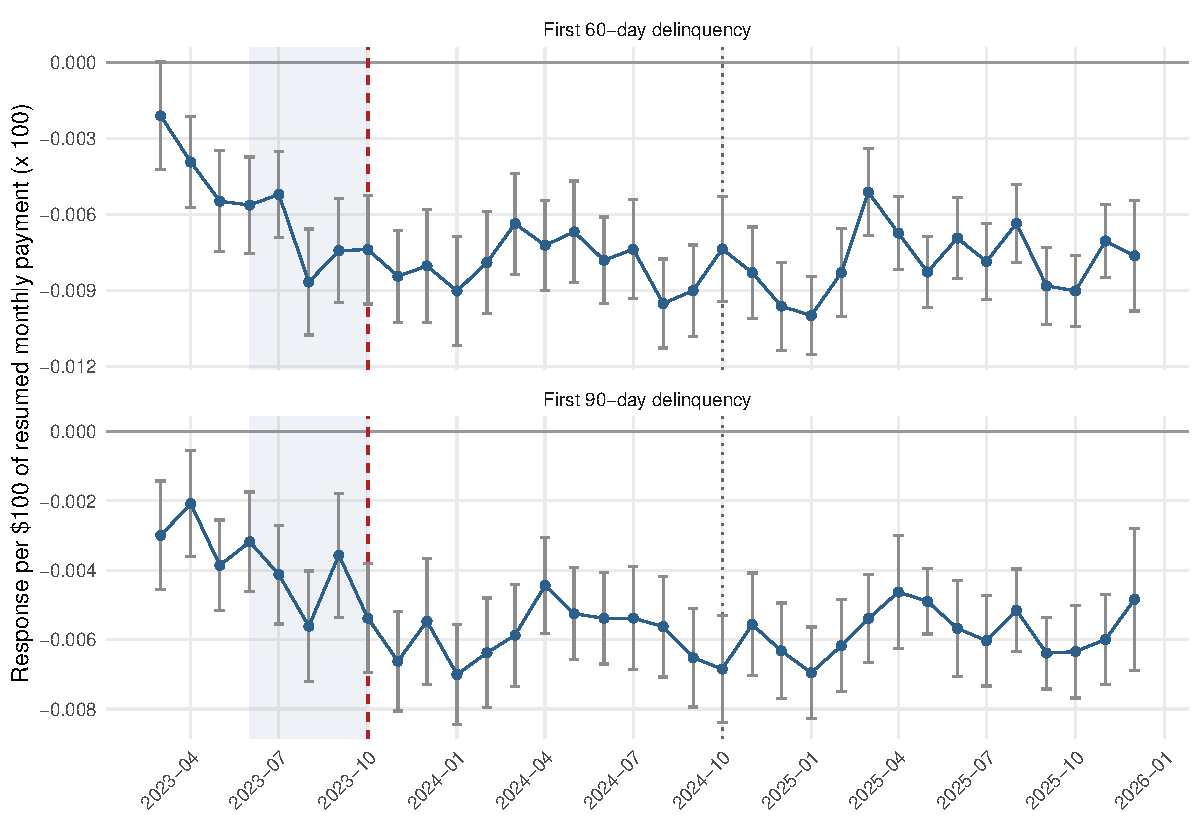
\includegraphics[width=0.95\textwidth]{figures/fig_student_profile.pdf}
\caption{Auto-loan delinquency and the resumed student-loan bill. Coefficients ($\times 100$) of first 90-day and 60-day delinquency on the resumed monthly bill in hundreds of dollars, by calendar month, with loan and month fixed effects; reference January 2022 to February 2023; 95 percent bands. Shaded: the four months between the statute of 3 June 2023 and the first bill; dashed: October 2023; dotted: the end of the on-ramp, October 2024.}
\label{fig:student_profile}
% replication: Code/extract/E13_student_resumption.R, Code/identification/I11_student_resumption.R, Code/exhibits/make_student_figures.R
\end{figure}

\begin{table}[H]
\centering
\caption{Take-up of the resumed student-loan bills}
\label{tab:student_takeup}
\small
\resizebox{\textwidth}{!}{\begin{tabular}{lrrrrrrrrr}
\toprule
Resumed bill & Holders & \multicolumn{2}{c}{2023-11} & \multicolumn{2}{c}{2024-01} & \multicolumn{2}{c}{2024-10} & \multicolumn{2}{c}{2025-01} \\
\cmidrule(lr){3-4}\cmidrule(lr){5-6}\cmidrule(lr){7-8}\cmidrule(lr){9-10}
 & (2023-09) & Paying & Past due & Paying & Past due & Paying & Past due & Paying & Past due \\
\midrule
Zero & 149,088 & 0.03 & 0.008 & 0.04 & 0.007 & 0.08 & 0.011 & 0.10 & 0.012 \\
\$1--100 & 83,372 & 0.31 & 0.019 & 0.41 & 0.018 & 0.36 & 0.017 & 0.36 & 0.019 \\
\$101--250 & 92,512 & 0.43 & 0.020 & 0.55 & 0.020 & 0.49 & 0.020 & 0.50 & 0.022 \\
\$251--500 & 61,295 & 0.50 & 0.026 & 0.60 & 0.026 & 0.55 & 0.025 & 0.55 & 0.027 \\
More than \$500 & 43,651 & 0.55 & 0.043 & 0.61 & 0.044 & 0.57 & 0.041 & 0.56 & 0.042 \\
\bottomrule
\end{tabular}
}
\vspace{0.5em}
\begin{minipage}{0.92\textwidth}
\noindent \small \textit{Notes:} Holders of a positive federal student-loan balance in September 2023, by the resumed monthly bill. Actual payment: the share with a positive actual-payment amount on any student trade in the month; ratio: the median of actual to scheduled payment among all holders in the bin; past due: the share with a positive past-due student balance.
\end{minipage}
% replication: Code/extract/E13b_student_takeup.R
\end{table}

\begin{table}[H]
\centering
\caption{The response to the resumed bill by group}
\label{tab:student_groups}
\small
\resizebox{\textwidth}{!}{\begin{tabular}{llrrrrrrr}
\toprule
Outcome & Group & Loans & Events & Base & Before (Jun--Sep 2023) & At (Oct--Dec 2023) & After (2024--25) & Ratio \\
\midrule
90-day & All  & 738,722 & 17,711 & 0.066 & -0.004 (0.000) & -0.005 (0.000) & -0.005 (0.000) & 0.68 \\
90-day & Score tercile 1 & 256,441 & 13,837 & 0.157 & -0.003 (0.001) & -0.006 (0.002) & -0.005 (0.001) & 0.62 \\
90-day & Score tercile 2 & 242,503 & 3,316 & 0.031 & -0.001 (0.001) & -0.003 (0.001) & -0.003 (0.000) & 0.50 \\
90-day & Score tercile 3 & 239,762 & 558 & 0.004 & -0.000 (0.000) & -0.001 (0.000) & -0.001 (0.000) & 0.44 \\
90-day & Income quartile 1 & 187,038 & 7,716 & 0.131 & -0.008 (0.001) & -0.009 (0.002) & -0.009 (0.001) & 0.86 \\
90-day & Income quartile 2 & 185,814 & 6,564 & 0.091 & 0.001 (0.002) & -0.006 (0.002) & -0.004 (0.001) & -0.10 \\
90-day & Income quartile 3 & 181,150 & 2,529 & 0.029 & -0.001 (0.001) & 0.001 (0.001) & -0.001 (0.000) & -0.64 \\
90-day & Income quartile 4 & 178,412 & 780 & 0.008 & -0.000 (0.000) & -0.000 (0.000) & -0.000 (0.000) & 3.50 \\
60-day & All  & 733,653 & 28,742 & 0.124 & -0.006 (0.001) & -0.007 (0.001) & -0.007 (0.000) & 0.83 \\
60-day & Score tercile 1 & 257,787 & 21,831 & 0.290 & -0.006 (0.002) & -0.005 (0.002) & -0.007 (0.001) & 1.21 \\
60-day & Score tercile 2 & 239,790 & 5,795 & 0.060 & -0.003 (0.001) & -0.005 (0.001) & -0.005 (0.000) & 0.57 \\
60-day & Score tercile 3 & 236,060 & 1,116 & 0.010 & -0.000 (0.000) & -0.001 (0.000) & -0.001 (0.000) & 0.24 \\
60-day & Income quartile 1 & 186,638 & 11,463 & 0.222 & -0.010 (0.002) & -0.010 (0.002) & -0.013 (0.001) & 0.97 \\
60-day & Income quartile 2 & 185,493 & 10,807 & 0.179 & -0.005 (0.002) & -0.006 (0.002) & -0.005 (0.001) & 0.92 \\
60-day & Income quartile 3 & 179,410 & 4,661 & 0.066 & 0.001 (0.001) & -0.001 (0.001) & -0.001 (0.001) & -0.60 \\
60-day & Income quartile 4 & 175,861 & 1,652 & 0.020 & -0.001 (0.000) & -0.001 (0.000) & -0.001 (0.000) & 0.44 \\
\bottomrule
\end{tabular}
}
\vspace{0.5em}
\begin{minipage}{0.92\textwidth}
\noindent \small \textit{Notes:} Coefficients ($\times 100$) of first delinquency on the resumed bill in hundreds of dollars interacted with three windows, June to September 2023 (before the first bill), October to December 2023 (at it) and January 2024 onward (after it), with loan and calendar-month fixed effects; standard errors clustered by consumer; base: the monthly hazard in the reference window, percent. Ratio: before over at. Score and income at the auto loan's first sight in the panel.
\end{minipage}
% replication: Code/identification/I11_student_resumption.R
\end{table}

